\begin{docTcbKey}{lefthand width}{=\meta{length}}{no default, initially unset}

Sets the width of the left-handed part to the given \meta{length}.

将左部的宽度设置为给定的\meta{length}。


\begin{dispExample}
\tcbset{colback=red!5!white,colframe=red!75!black,fonttitle=\bfseries}

\begin{tcolorbox}[title=My title,sidebyside,lefthand width=3cm]
这是 upper (\textit{左}) 部分.
\tcblower
这是 lower (\textit{右}) 部分.
\end{tcolorbox}
\end{dispExample}
\end{docTcbKey}

\enlargethispage*{1cm}
\begin{docTcbKey}{righthand width}{=\meta{length}}{no default, initially unset}

Sets the width of the right-handed part to the given \meta{length}.

将右部的宽度设置为给定的\meta{length}。


\begin{dispExample}
\tcbset{colback=red!5!white,colframe=red!75!black,fonttitle=\bfseries}

\begin{tcolorbox}[title=My title,sidebyside,righthand width=3cm]
这是 upper (\textit{左}) 部分.
\tcblower
这是 lower (\textit{右}) 部分.
\end{tcolorbox}
\end{dispExample}
\end{docTcbKey}

% \clearpage
\begin{docTcbKey}{lefthand ratio}{=\meta{fraction}}{no default, initially |0.5|}

Sets the width of the left-handed part to the given \meta{fraction} of
the available space. \meta{fraction} is a value between |0| and |1|.

设置左侧的宽度为所有可用宽度的比例 \meta{fraction}。
\meta{fraction} 取值在 |0| 到 |1|。


\begin{dispExample}
\tcbset{colback=red!5!white,colframe=red!75!black,fonttitle=\bfseries}

\begin{tcolorbox}[title=My title,sidebyside,lefthand ratio=0.25]
这是 upper (\textit{左}) 部分.
\tcblower
这是 lower (\textit{右}) 部分.
\end{tcolorbox}
\end{dispExample}
\end{docTcbKey}


\begin{docTcbKey}{righthand ratio}{=\meta{fraction}}{no default, initially |0.5|}

Sets the width of the right-handed part to the given \meta{fraction} of
the available space. \meta{fraction} is a value between |0| and |1|.

设置右侧的宽度为所有可用宽度的比例 \meta{fraction}。
\meta{fraction} 取值在 |0| 到 |1|。


\begin{dispExample}
\tcbset{colback=red!5!white,colframe=red!75!black,fonttitle=\bfseries}
\begin{tcolorbox}[title=My title,sidebyside,righthand ratio=0.25]
这是 upper (\textit{左}) 部分.
\tcblower
这是 lower (\textit{右}) 部分.
\end{tcolorbox}
\end{dispExample}
\end{docTcbKey}


% \clearpage

If one side of a side-by-side box should be adapted to the width of its content, 
this width has to be computed beforehand.
The following example uses a savebox |\mysavebox| to store the picture to determine its width. 
A more convenient way to handle this task is to use the methods from \Fullref{subsec:sidebyside_xparse}.

如果一个并排的盒子的一边要适应其内容的宽度, %
这个宽度必须事先计算。%
下面的例子使用一个存储盒子 |\mysavebox| 来存储图片以确定其宽度。%
处理这个任务更方便的方法是使用来自 \Fullref{subsec:sidebyside_xparse} 的方法。

\begin{引述之言}{virhuiai}
可以在code中处理,见下面的例子。
\end{引述之言}
% code={\sbox{\mysavebox}{#2}}, % lefthand width=\wd\mysavebox,

\begin{dispExample}
% \tcbuselibrary{skins,xparse}
% \usepackage{lipsum}
% \newsavebox\mysavebox  % preamble
\DeclareTotalTColorBox{\mysidebox}{ O{} +m +m }{
  bicolor,colback=white,colbacklower=yellow!10,
  fonttitle=\bfseries,center title,
  sidebyside,
  code={\sbox{\mysavebox}{#2}},
  lefthand width=\wd\mysavebox,
  drop lifted shadow,
  #1
}
{\usebox{\mysavebox}\tcblower#3}

\mysidebox[title=The Triangle]{%
  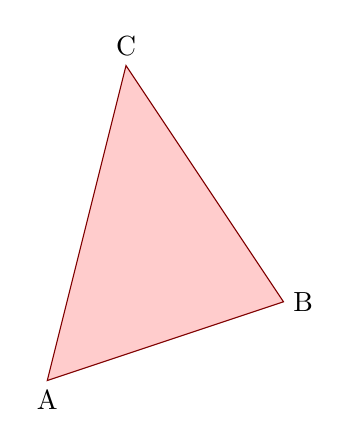
\begin{tikzpicture}
    \path[fill=red!20,draw=red!50!black]
      (0,0) node[below]{A} -- (3,1) node[right]{B}
      -- (1,4) node[above]{C} -- cycle;
  \end{tikzpicture}%
}{%
  \lipsum[1]
} 
\end{dispExample}